\chapter{Methodology}
% Hva er vurderinger basert på, subjektivt?
% Vurdere metodikken kritisk
% Vurdere kilder for innsamling. Hvordan ble disse brukt; søkeord, filtrering
% Vurdere innsamlingsmetoder og deres troverdighet
% Metodekritikk
% Viktig å få med hvorfor vi velger den metoden vi har valgt
% Viktig å få med at dette er et VELDIG bevisst valg.
% SYSTEMATISK
% beskrive metrikk, kriterier
% Beskrive begrepet og nøyaktig hvordan vi har tenkt å bruke det, inkl metrikker relatert til det.
This chapter will cover the description and choice of methods used in this bachelor thesis.
\section{Literary study}
The literary study that is to be conducted will constitute the main part of this project and will also be the foundation for the entirety of this bachelor thesis. Therefore, the methodology for this phase of the report is crucial.

\subsection{Information gathering}
This sub phase of the study will be the basis for each subsequent process. The result needs to be representative for the existing technologies as well as thorough. This process will span over roughly four weeks, and the result should represent roughly three months of work per team member. We consider this to be sufficient with regards to our scope. We categorised collected papers in four categories. This is to ease the prioritisation of reading. These four categories are as follows:

\begin{description}
    \item [Useful:] The \textit{useful} category contains information which we have deemed directly useful to the completion of this paper.
    \item [Relevant:] The \textit{relevant} information contains information which we have deemed relevant, but not directly includeable.
    \item [Interesting:] The \textit{interesting} category contains information which we have deemed to be interesting to the area of research and that may lead to interesting perspectives or contain \textit{relevant} or \textit{useful} references.
    \item [Less Relevant:] The \textit{less relevant} category contains information that we have deemed to be less relevant to our direct project, but may contain references to other \textit{useful}, \textit{interesting} or \textit{relevant} information.
\end{description}

\subsection{Analysis}
\label{2.1.2: Analysis_chap}

% Må prøve å finne referanser og underbygge kriteriene
\subsubsection{Criteria for evaluating technologies}
These criteria derive from consulting with our contact at Kongsberg Defence \& Aerospace, a former employee of the Norwegian defence, and our own deduction. Therefore, these criteria are expert opinions and subjective.

\begin{description}
    \item[Availability:] In a tactical environment information like orders or fire commands must be transmitted and received within a certain window of opportunity to be acted upon. This sets availability to be an important factor in these networks. Therefore, a technology for authentication should not alter availability in ways that lead to bad availability.
    
    In certain tactical situations there even may be willingness to accept a breach of security specifications on behalf of a need to send important information. This means it becomes more important to alert the breach instead of actually stopping the process. Therefore, there may be a need to evaluate the possibilities at a given time regarding the balance between security and availability.
  
    \item[Autonomous system with graceful degradation:] By military standards, if a node gets compromised or lose connection it should not affect the rest of the networks functionality. Therefore, such a system needs to have a degree of autonomousity. For authentication, this may be each component is able to authenticate into the network with bootstrapped credentials the other nodes can verify. Another case with the use of groups, another way may be capabilities to remediate changes to the group structure. This means, if one is lost there should be ways to restore the functionality of the group.

    \item[Security:] For military purposes, tactical communication should not be compromised within an operative window, meaning window of opportunity to act on, for example, an order. Authentication is one of the mechanisms that affect the outcome of such cases. This is done by only allowing authenticated devices to communicate through established encrypted channels. Therefore, the process of authenticating needs to be secure in itself to have trust in the integrity of communication.

    \item[Resource consumption:] The tactical environment in question often consist of varying infrastructure and quality of service. The bandwidth may put restraints on how much negotiation between nodes can be justified. The authentication processes should not halt the networks main purpose, to send and receive data. Therefore, the amount of traffic generated from the authentication will be analysed.

    \item[Loss-tolerant:] Substantial amounts of overhead and negotiation may be problematic if the network is prone to packet loss. This may be cause of fleeting availability or packet dropping due to network congestion. Therefore, we will analyse whether the technologies have capabilities for loss-tolerance.

    \item[Degree of automation:] In a tactical situation it is preferred to have technology which have a low level of interaction to make it function. This may favor technology which rely on bootstrapping the devices to function immediately without any setup by the end user.
\end{description}
\subsection{Taxonomy and Classification}
\begin{figure}[!h]
    \label{uvmodel}
    \centering
    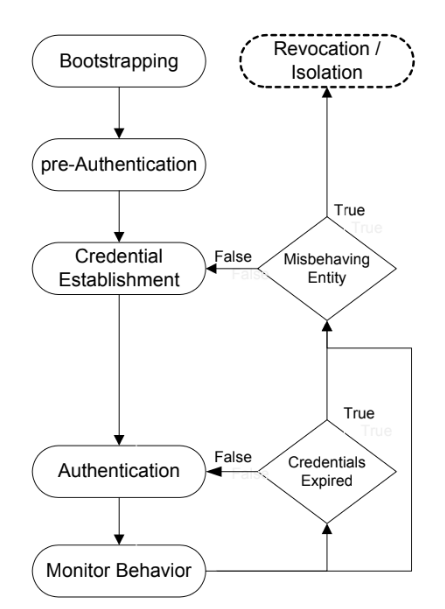
\includegraphics[scale=0.5]{appendices/Authentication_flow_chart.png}
    \caption{Generic Authentication flow \cite{DBLP:conf/mswim/AboudaggaREDQ05}}
\end{figure}

\begin{figure}[!h]
    \label{uvmodel}
    \centering
    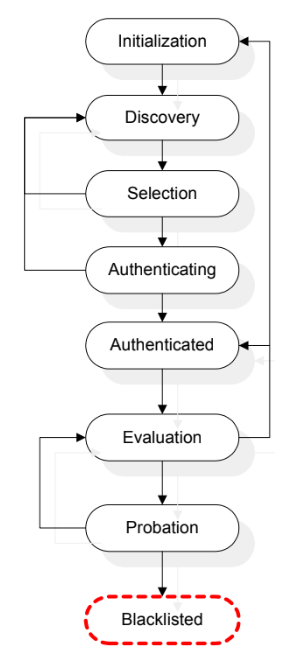
\includegraphics[scale=0.5]{appendices/Node_Authentication_States.png}
    \caption{Node Authentication States \cite{DBLP:conf/mswim/AboudaggaREDQ05}}
\end{figure}

\subsection{Discussion}

\textit{\textbf{Discussion}} will be a crucial part of the literary study. In this sub-phase, the technologies will be compared and contrasted based on the findings from the \textit{Analysis} phase. The pertinent point of this phase is to directly see how different technologies compare in relation to each others with respects to the relevant metrics and specifications.

